
\section{Базовый алгоритм}

Первый алгоритм, который мы рассмотрим -- это алгоритм Дейкстры. Он позовляет вычислять кратчайшие рассточния от $s \in V$ до всех вершин в графе, если у нас неотрицательная весовая функция. Далее считаем, что \textit{весовая функция неотрицательна}.

\begin{algorithm}[H]
\caption{Алгоритм Дейкстры}
\begin{algorithmic}[1]

\Function{dijkstra}{$G, w, s$}
    \State $\delta_c(s, v) = +\infty, \forall v \in V$
    \State $\delta_c(s, s) = 0$
    \State $K = \{ s \}$ \Comment{Множество вершин, до которых мы знаем расстояние.}

    \While{$K \neq V$}
        \State $u \gets \argmin\limits_{v \in V \backslash K} \delta_c(s, v)$ \Comment{Получаем вершину из неизвестных с минимальным $\delta$}
        \State $K \gets K \cup \{ u \}$ \Comment{Утверждается, что для $u$ $\delta$ посчитана корректна (док-во см. далее)}

        \For{$v \in \alpha(u)$}
            \State $\delta_c(s, v) \gets \min \{\delta_c(s, v), \delta_c(s, u) + w(u, v)\}$
        \EndFor
    \EndWhile

    \State \Return $\delta_c$
\EndFunction
\end{algorithmic}
\end{algorithm}

\Def Обновление $\delta_c$ в строчках 8-9 будем называть \textit{релаксацией}.

\section{Корректность}

Далее приведем доказательство корректности, но перед этим докажем мини-лемму. Далее под $\delta_c$ будем понимать <<расстояния>> из алгоритма выше. В последтвии мы покажем, что $\delta_c \equiv \delta$.

\Lm $\forall v \in V \hookrightarrow \delta(s, v) \leq \delta_c(s, v)$

\begin{proof}
    В силу 9-ой строчки алгоритма $\exists v_1 \in V: \delta_c(s, v_0) = \delta_c(s, v_1) + w(v_1, v_0)$ (то есть раньше была какая-то вершина, из которой мы произвели релаксацию $v_0$). Но также мы можем сказать и про $v_1$, действительно, $\exists v_2 \in V: \delta_c(s, v_1) = \delta_c(s, v_2) + w(v_2, v_1)$. Итого:
    \begin{equation*}
        \delta_c(s, v_0) = \delta_c(s, v_2) + w(v_2, v_1) + w(v_1, v_0)
    \end{equation*}
    Будем применять последовательно рассуждения выше к $\delta_c$, пока не дойдем до $s$, и получим, что:
    \begin{equation*}
        \delta_c(s, v_0) = \sum\limits_{k=1}^{m} w(v_{k}, v_{k - 1}), v_m = s
    \end{equation*}
    Значит, мы нашли путь $P_0 = \{s \rightarrow v_{m - 1} \rightarrow v_{m - 2} \rightarrow \dots \rightarrow v_0\}$ с весом $\delta_c(s, v_0)$. Далее воспользуемся определением $\delta$ и получим требуемое:
    \begin{equation*}
        \delta(s, v_0) \overset{def}{=} \min\limits_{P} w(P) \leq w(P_0) = \delta_c(s, v_0)
    \end{equation*}
    \begin{equation*}
        \delta(s, v_0) \leq \delta_c(s, v_0)
    \end{equation*}
\end{proof}

\Th $\delta_c \equiv \delta$, то есть получившиеся на выходе расстояния корректно посчитаны.
\begin{proof}

Покажем по индукции, что утверждение верно. Начнем с базы, а именно с начальной вершины. Действительно, $\delta_c(s, s) = 0 = \delta(s, s)$.

Пусть на 6-ой строчке алгоритма мы достаём вершину $t$. Предположим $\delta(s, t) \neq \delta_c(s, t)$, т.е. $\exists P$ - кратчайший путь, т.ч. $w(P) < \delta_c(s, t)$. На этом пути возьмем самую первую вершину $v$ такую, что $v \in V \backslash K$. Далее возьмем ей предшествующую $u$. Ясно, что $u \in K$, по определению $v$.

\begin{figure}[H]
\centering
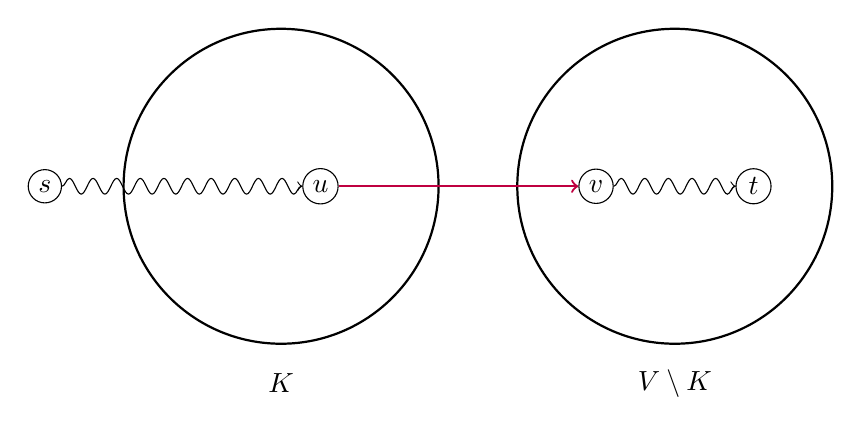
\begin{tikzpicture}[
    node distance=2cm,
    every node/.style={circle, draw, inner sep=2pt},
    decoration={snake, amplitude=1mm, segment length=3mm}
]
    % Большие круги
    \draw[thick] (0,0) circle (2cm);
    \draw[thick] (5,0) circle (2cm);
    
    % Подписи
    \node[draw=none, rectangle] at (0,-2.5) {$K$};
    \node[draw=none, rectangle] at (5,-2.5) {$V \setminus K$};
    
    % Узлы
    \node (s) at (-3,0) {$s$};
    \node (u) at (0.5,0) {$u$};
    \node (v) at (4,0) {$v$};
    \node (t) at (6,0) {$t$};
    
    % Стрелки
    \draw[->, decorate, decoration=snake] (s) to[out=0,in=180] (u);
    \draw[->, purple, thick] (u) -- (v);
    \draw[->, decorate, decoration=snake] (v) to[out=0,in=180] (t);
\end{tikzpicture}

\caption{Предположение, что существует другой более короткий путь}
\label{fig:cut}
\end{figure}
В силу кратчайшести $P$, кратчайшим является, в частности, путь $s \rightsquigarrow v$. А значит:
\begin{equation*}
    \delta(s, v) = \delta(s, u) + w(u, v)
\end{equation*}
Комбинируя равенство выше, 9-ую строчку алгоритма и $\delta_c(s, u) = \delta(s, u)$ (см. предположение):
\begin{equation*}
    \delta_c(s, v) \leq \underbrace{\delta_c(s, u)}_{\delta(s, u)} + w(u, v) = \delta(s, u) + w(u, v) = \delta(s, v)
\end{equation*}
Значит:
\begin{equation*}
    \delta_c(s, v) \leq \delta(s, v)
\end{equation*}
Но по вышедоказанной лемме:
\begin{equation*}
    \delta(s, v) \leq \delta_c(s, v) \leq \delta(s, v) \Rightarrow \delta(s, v) = \delta_c(s, v)
\end{equation*}
Далее, коль скоро мы достаём вершину $t$, значит, у неё минимальное $\delta_c$ из всех, а значит $\delta_c(s, t) \leq \delta_c(s, v)$. Учитывая вышедоказанное, верно:
\begin{equation*}
    \delta_c(s, t) \leq \delta_c(s, v) = \delta(s, v)
\end{equation*}
Но вспомним, что $v$ стоит раньше $t$ в кратчайшем пути из $s$ в $t$, значит $\delta(s, v) \leq \delta(s, t)$ (см. картинку для наглядности). Значит:
\begin{equation*}
    \delta_c(s, t) \leq \delta(s, v) \leq \delta(s, t)
\end{equation*}
\begin{equation*}
    \delta_c(s, t) \leq \delta(s, t)
\end{equation*}
Но снова применяя вышедоказанную лемму, получаем требуемое противоречие с тем, что $\delta(s, t) \neq \delta_c(s, t)$:
\begin{equation*}
    \delta(s, t) \leq \delta_c(s, t) \leq \delta(s, t) \Rightarrow \delta(s, t) = \delta_c(s, t)
\end{equation*}

\end{proof}

Теперь рассмотрим время работы алгоритма. Заметим, что каждую вершину мы берём ровно один раз (время выбора зависит от реализации, обозначим его пока за $\tau(n)$). Далее, каждое ребро мы тоже смотрим ровно один раз и обновляем в цикле релаксации вершину за время $\eta(n)$. Значит, общее время работы: $\Theta(|V| \tau(|V|) + |E| \eta(|V|))$.

Рассмотрим теперь стратегии выбора вершины с минимальным $\delta_c$:
\begin{enumerate}
    \item Наивно. Просто ищем минимум в массиве всех вершин за $\Theta(|V|)$, а обновление в цикле релаксации -- это $\Theta(1)$. Тогда итоговая асимптотика $\Theta\left(|V|^2 + |E|\right)$.
    \item Двоичная куча. Поиск минимума -- $\O(\log |V|)$, обновление тоже $\O(\log |V|)$. Итоговая асимптотика $\O(|V| \log |V| + |E| \log |V|)$. Но, вспомним, что $|V| = \O(|E|)$, поэтому $\O(|V| \log |V| + |E| \log |V|) = \O(|E| \log |V|)$. Итого $\O(|E| \log |V|)$.
\end{enumerate}

\Note Вообще говоря, асимптотика еще зависит от способа хранения графа, кардинально они не меняются, но, например, если мы реализовали хранение графа в виде хеш-таблицы, то асимптотики будут уже \textit{в среднем} смысле.

Пусть теперь мы хотим найти кратчайшее расстояние от вершины $s$ до некоторой вершины $t$. Следующее следствие из теоремы даёт способ рассчета $\delta(s, t)$.

\Cons Пусть $t \in V$. Тогда чтобы найти $\delta(s, t)$, достаточно завершить алгоритм Дейкстры в момент, когда на 6-ой строчке была получена вершина $t$.

\section{Эвристический подход}

Давайте немного подробнее рассмотрим алгоритм Дейкстры и улучшим решение задачи нахождения $\delta(s, t)$. Если взять алгоритм как есть, то при достаточно плохом графе <<зона поиска>> будет достаточно большой.

И напрашивается такая мысль, что быть может не всегда оптимально так наивно перебирать вершины, и использовать какие-то общие приземленные данные о задаче и как-то это отразить в весовой функции, чтобы приотизировать выбор некоторых рёбер. Такие соображения о задаче называют \textit{эвристическими}.

\Def Функцию $h: V^2 \to \R^+$ будем называть эвристикой.

Теперь интегрируем нашу эвристику в алгоритм Дейкстры (такой алгоритм назвается $A^*$):

\begin{algorithm}[H]
\caption{Алгоритм $A^*$}
\begin{algorithmic}[1]

\Function{astar}{$G, w, s, t, h$}
    \State $\delta_c(s, v) = +\infty, \forall v \in V$
    \State $\delta_c(s, s) = 0$
    \State $K = \{ s \}$

    \While{$K \neq V$}
        \State $u \gets \argmin\limits_{v \in V \backslash K} [\delta_c(s, v) + h(v, t)]$ \Comment{Заметьте, что здесь используется эвристика}

        \If {$u = t$}
            \State \Return $\delta_c(s, u)$
        \EndIf
        
        \State $K \gets K \cup \{ u \}$

        \For{$v \in \alpha(u)$}
            \State $\delta_c(s, v) \gets \min \{\delta_c(s, v), \delta_c(s, u) + w(u, v)$\}
        \EndFor
    \EndWhile

    \State \Return $\delta_c$
\EndFunction
\end{algorithmic}
\end{algorithm}

Теперь встаёт вопрос о том какие вообще эвристические функции мы можем брать, ведь если взять достаточно плохую функцию $h$, то можно заставить алгоритм $A^*$ работать дольше Дейкстры или вообще сходиться к неверному ответу.

\Def Пусть $t \in V$. Эвристику $h$ будем называть \textit{допустимой}, если $\forall v \in V \hookrightarrow h(v, t) \leq \delta(v, t)$.

\Note Допустимость эвристики напрямую зависит от пункта назначения.

Далее приведём базовое утверждение, которое на экзамене будет без доказательства (но для интересующегося темой читателя оно приведено).

\ThBd Если эвристика допустима, то $A^*$ вернет верный результат, т.е. найдет оптимальный путь.

\begin{proof}
    Предположим противное. Пусть $A^*$ вернул неверный результат $\delta^*$. Ясно, что $\delta(s, t) < \delta^*$.
    Заметим, что доколе алгоритм работает, то в $K$ обязана находиться хотя бы одна вершина $v$, которая находится на оптимальном пути до $t$. Пусть это не так, значит в частности нет и $t$, ведь, очевидно, $t$ лежит на таком пути. Коль скоро $v$ лежит на оптимальном пути, $\delta(s, t) = \delta(s, v) + \delta(v, t)$ (предлагается это читателю доказать, как простое логическое упражнение). В силу допустимости эвристики заключаем:
    \begin{equation*}
        \delta(s, v) + h(v, t) \leq \delta(s, v) + \delta(v, t) = \delta(s, t)
    \end{equation*}
    \begin{equation*}
        \delta_c(s, v) + h(v, t) \leq \delta(s, v) + h(v, t) \leq \delta(s, t)
    \end{equation*}
    \begin{equation*}
        \delta_c(s, v) + h(v, t) \leq \delta(s, t)
    \end{equation*}
    Заметим, что $h(t, t) \leq \delta(t, t) = 0 \Rightarrow h(t, t) = 0 \Rightarrow \delta_c(s, t) = \delta_c(s, t) + h(t, t)$. По вышедоказанной лемме:
    \begin{equation*}
        \delta(s, t) \leq \delta_c(s, t) = \delta_c(s, t) + h(t, t)
    \end{equation*}
    Далее:
    \begin{equation*}
        \delta_c(s, v) + h(v, t) \leq \delta(s, t) \leq \delta_c(s, t) + h(t, t)
    \end{equation*}
    \begin{equation*}
        \delta_c(s, v) + h(v, t) \leq \delta_c(s, t) + h(t, t)
    \end{equation*}
    Значит, мы не вытащим вершину $t$, пока не вытащим из $K$ все вершины находящиеся на оптимальном пути (см. определение вершины $v$), а найденное $\delta_c(s, t)$ будет валидно посчитано.
\end{proof}

\Def Эвристику $h$ будем называть монотонной, если $\forall (u, v) \in E \hookrightarrow h(u, t) - h(v, t) \leq w(u, v)$ и $h(t, t) = 0$.

\St Всякая монотонная эвристика допустима.

\begin{proof}
    Покажем корректность утверждения по индукции по рёберной длине.

    База. $0 = h(t, t) \leq \delta(t, t) = 0$.

    Переход. Пусть показали для длины $n_0 - 1$, покажем для $n_0$. Возьмем вершину $t$ такой что до неё расстояние от $s$ равно $n_0$. Тогда возьмем вершину на кратчайшем пути перед $t$ на расстоянии $n_0 - 1$ рёбер -- $v$ (то есть из вершины $s$ до $v$ есть ребро). Значит для вершины $v$ можем применить предположение индукции: $h(v, t) \leq \delta(v, t)$. Комбинируя с тем, что $h(s, t) - h(v, t) \leq w(s, v)$ получаем требуемое:
    \begin{equation*}
        h(s, t) \leq w(s, v) + h(v, t) \leq w(s, v) + \delta(v, t) = \delta(s, t)
    \end{equation*}
\end{proof}

\ThBd Если эвристика монотонна, то алгоритм $A^*$ выдает корректный результат и работает по времени не медленнее, чем алгоритм Дейкстры.